% ProfileXAI — Diagrama de Arquitectura del Sistema
\documentclass[a3paper,landscape]{article}
\usepackage[margin=1.8cm]{geometry}
\usepackage{tikz}
\usepackage[T1]{fontenc}
\usepackage[utf8]{inputenc}
\usepackage{lmodern}
\usetikzlibrary{
  shapes.geometric, arrows.meta, positioning,
  fit, backgrounds, shadows.blur, calc
}

% ── Paleta de colores ───────────────────────────────────────────────────────
\definecolor{clrFront}{HTML}{2563EB}   % azul frontend
\definecolor{clrBack}{HTML}{059669}    % verde backend
\definecolor{clrDocker}{HTML}{D97706}  % naranja docker
\definecolor{clrXAI}{HTML}{DB2777}     % rosa XAI
\definecolor{clrRAG}{HTML}{7C3AED}     % violeta RAG
\definecolor{clrStore}{HTML}{475569}   % gris storage
\definecolor{clrJob}{HTML}{0284C7}     % azul job store

\definecolor{bgFront}{HTML}{EFF6FF}
\definecolor{bgBack}{HTML}{ECFDF5}
\definecolor{bgDocker}{HTML}{FFFBEB}
\definecolor{bgXAI}{HTML}{FDF2F8}
\definecolor{bgRAG}{HTML}{F5F3FF}
\definecolor{bgStore}{HTML}{F1F5F9}
\definecolor{bgJob}{HTML}{E0F2FE}
\definecolor{bgUser}{HTML}{F0FDF4}

% ── Estilos ─────────────────────────────────────────────────────────────────
\tikzset{
  % Caja genérica
  box/.style={
    rectangle, rounded corners=5pt,
    minimum width=#1, minimum height=0.75cm,
    text centered, font=\footnotesize\bfseries,
    blur shadow={shadow blur steps=5, shadow xshift=1pt, shadow yshift=-1pt}
  },
  box/.default=3cm,
  % Caja de subcomponente pequeño
  sub/.style={
    rectangle, rounded corners=3pt,
    minimum width=2.8cm, minimum height=0.6cm,
    text centered, font=\scriptsize,
    draw, inner sep=3pt
  },
  % Flechas principales
  flow/.style={-{Stealth[length=7pt]}, line width=1.4pt},
  flowdash/.style={-{Stealth[length=7pt]}, line width=1pt, dashed},
  % Etiqueta de flecha
  lbl/.style={font=\scriptsize, midway, fill=white, inner sep=2pt}
}

% ── Separador de sección (bloque de título lateral) ─────────────────────────
\newcommand{\seclabel}[3]{%
  \node[rotate=90, font=\footnotesize\bfseries, text=#3] at (#1) {#2};
}

\begin{document}
\pagestyle{empty}
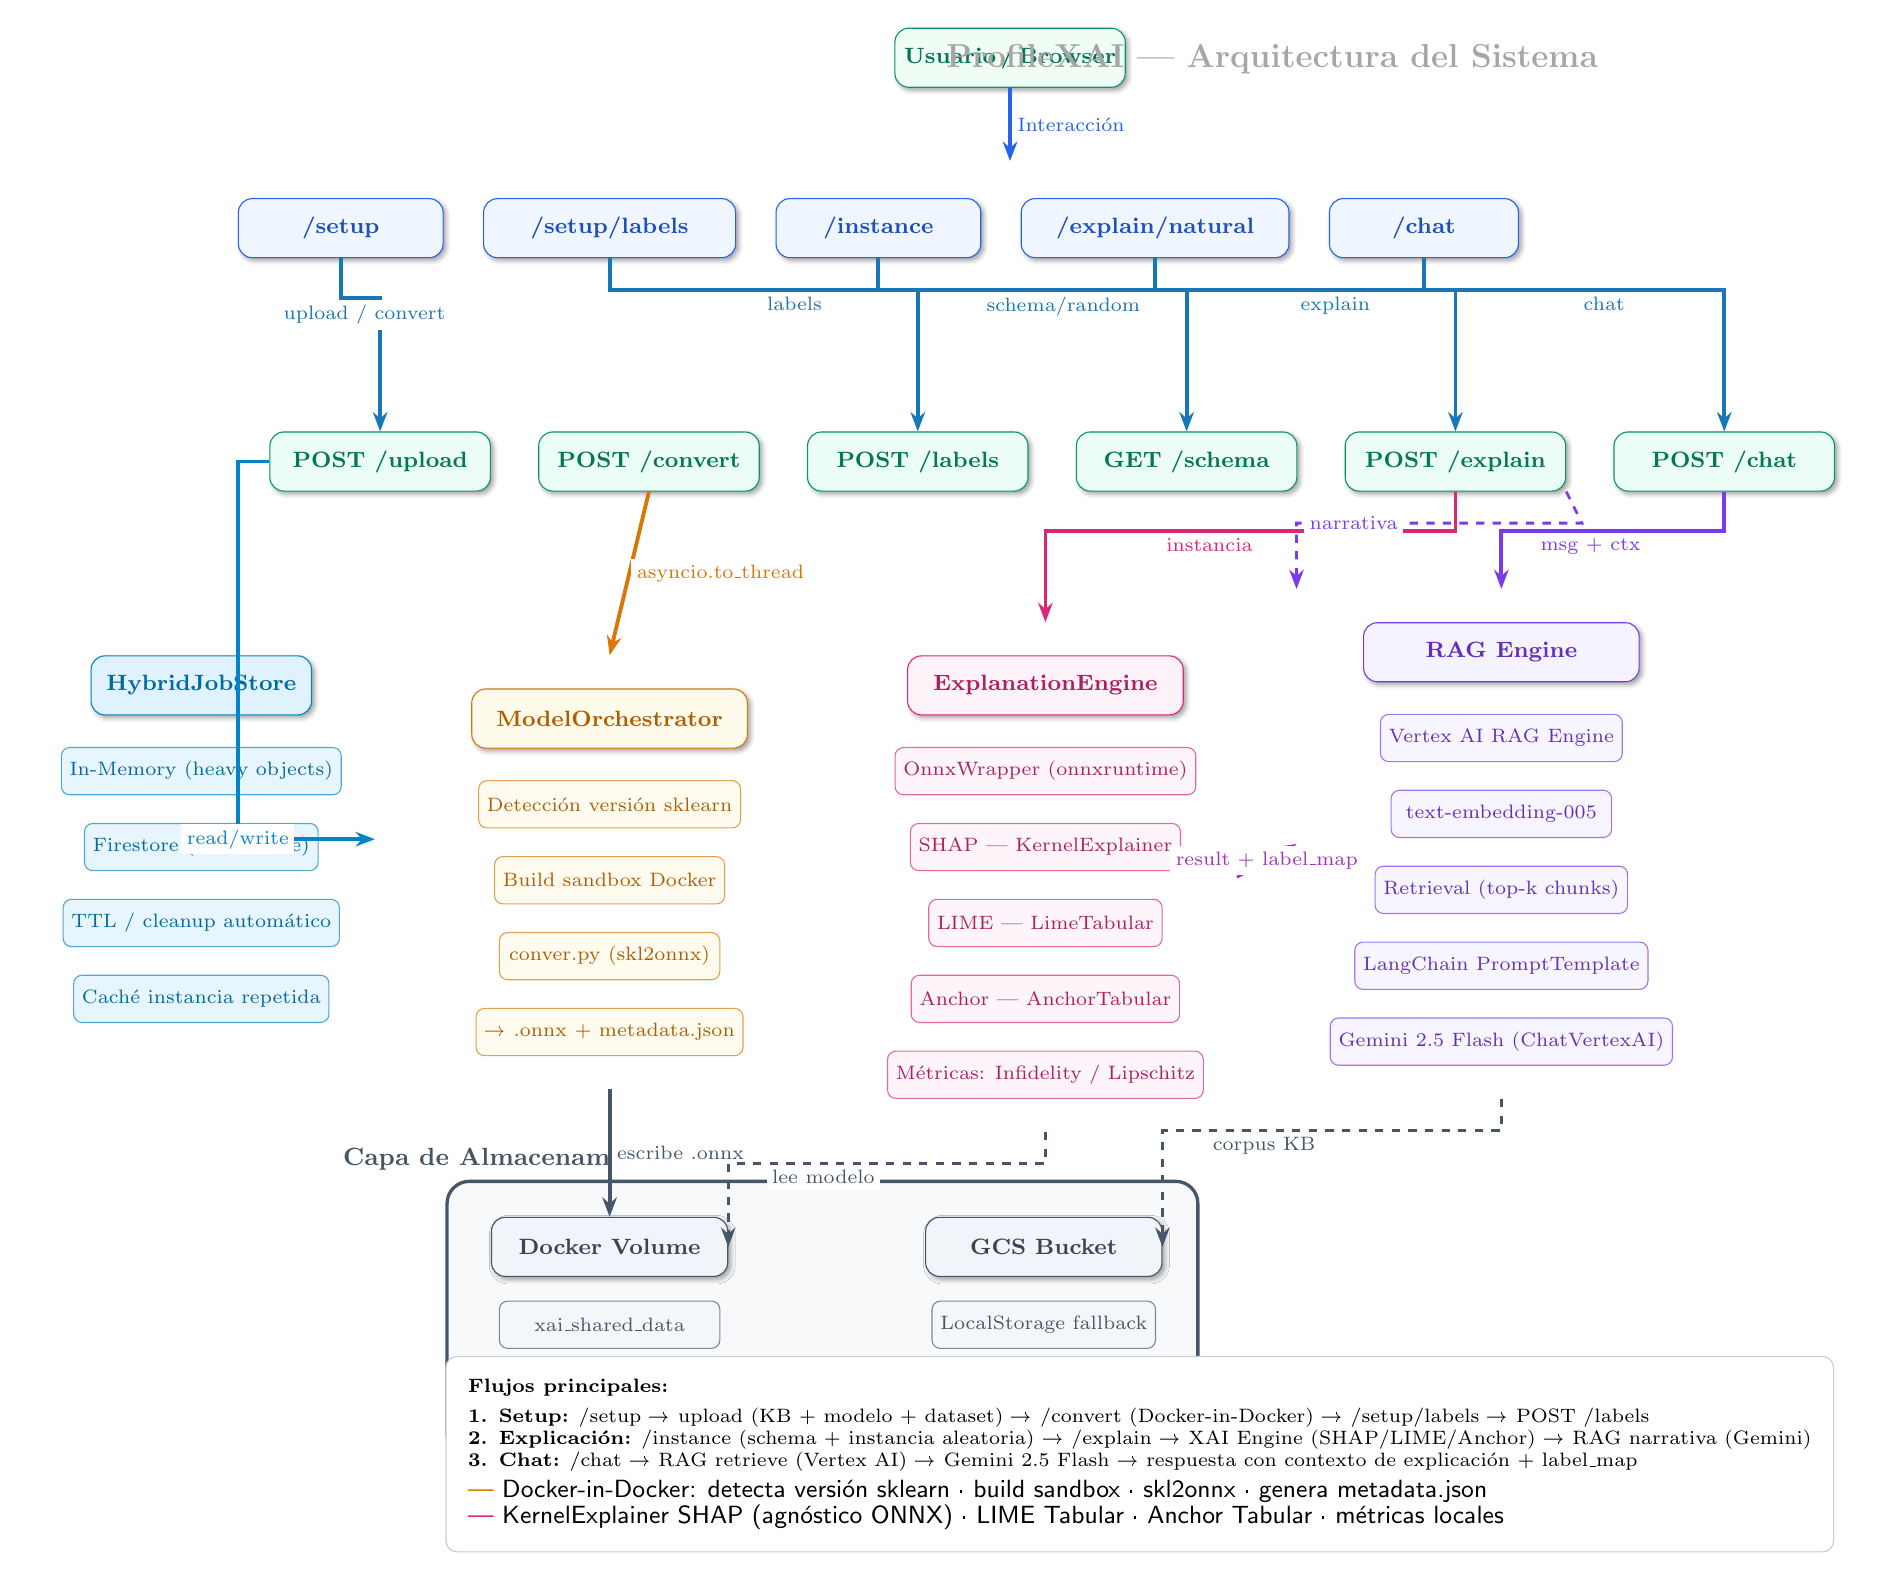
\begin{tikzpicture}[node distance=0.9cm and 1.1cm]

%% ═══════════════════════════════════════════════════════════════════════════
%% FILA 0 — USUARIO
%% ═══════════════════════════════════════════════════════════════════════════
\node[box=2cm, fill=bgUser, draw=clrBack, text=clrBack!80!black] (user) {Usuario\,/\,Browser};

%% ═══════════════════════════════════════════════════════════════════════════
%% FILA 1 — FRONTEND (Next.js)
%% ═══════════════════════════════════════════════════════════════════════════
\node[box=2.6cm, fill=bgFront, draw=clrFront, text=clrFront!80!black,
      below=1.4cm of user, xshift=-8.5cm] (pg_setup) {/setup};
\node[box=3.2cm, fill=bgFront, draw=clrFront, text=clrFront!80!black,
      right=0.5cm of pg_setup] (pg_labels) {/setup/labels};
\node[box=2.6cm, fill=bgFront, draw=clrFront, text=clrFront!80!black,
      right=0.5cm of pg_labels] (pg_instance) {/instance};
\node[box=3.4cm, fill=bgFront, draw=clrFront, text=clrFront!80!black,
      right=0.5cm of pg_instance] (pg_explain) {/explain/natural};
\node[box=2.4cm, fill=bgFront, draw=clrFront, text=clrFront!80!black,
      right=0.5cm of pg_explain] (pg_chat) {/chat};

% Marco del layer frontend
\begin{scope}[on background layer]
  \node[draw=clrFront, line width=1.2pt, fill=bgFront!60,
        rounded corners=8pt, inner sep=0.45cm,
        fit=(pg_setup)(pg_labels)(pg_instance)(pg_explain)(pg_chat),
        label={[clrFront, font=\small\bfseries]above left:Frontend — Next.js \texttt{:3000}}]
        (frontend_box) {};
\end{scope}

%% ═══════════════════════════════════════════════════════════════════════════
%% FILA 2 — BACKEND (FastAPI)
%% ═══════════════════════════════════════════════════════════════════════════
\node[box=2.8cm, fill=bgBack, draw=clrBack, text=clrBack!80!black,
      below=2.2cm of pg_setup, xshift=0.5cm] (ep_upload) {POST /upload};
\node[box=2.8cm, fill=bgBack, draw=clrBack, text=clrBack!80!black,
      right=0.6cm of ep_upload] (ep_convert) {POST /convert};
\node[box=2.8cm, fill=bgBack, draw=clrBack, text=clrBack!80!black,
      right=0.6cm of ep_convert] (ep_labels_ep) {POST /labels};
\node[box=2.8cm, fill=bgBack, draw=clrBack, text=clrBack!80!black,
      right=0.6cm of ep_labels_ep] (ep_schema) {GET /schema};
\node[box=2.8cm, fill=bgBack, draw=clrBack, text=clrBack!80!black,
      right=0.6cm of ep_schema] (ep_explain) {POST /explain};
\node[box=2.8cm, fill=bgBack, draw=clrBack, text=clrBack!80!black,
      right=0.6cm of ep_explain] (ep_chat) {POST /chat};

% Marco del layer backend
\begin{scope}[on background layer]
  \node[draw=clrBack, line width=1.2pt, fill=bgBack!60,
        rounded corners=8pt, inner sep=0.45cm,
        fit=(ep_upload)(ep_convert)(ep_labels_ep)(ep_schema)(ep_explain)(ep_chat),
        label={[clrBack, font=\small\bfseries]above left:Backend — FastAPI \texttt{:8000}}]
        (backend_box) {};
\end{scope}

%% ═══════════════════════════════════════════════════════════════════════════
%% FILA 3 — COMPONENTES CORE
%% ═══════════════════════════════════════════════════════════════════════════

%% ── Docker-in-Docker ───────────────────────────────────────────────────────
\node[box=3.5cm, fill=bgDocker, draw=clrDocker, text=clrDocker!80!black,
      below=2.5cm of ep_convert, xshift=-0.5cm] (dind_orch) {ModelOrchestrator};

\node[sub, fill=bgDocker!80, draw=clrDocker!70, text=clrDocker!80!black,
      below=0.4cm of dind_orch] (dind_detect) {Detección versión sklearn};
\node[sub, fill=bgDocker!80, draw=clrDocker!70, text=clrDocker!80!black,
      below=0.35cm of dind_detect] (dind_build) {Build sandbox Docker};
\node[sub, fill=bgDocker!80, draw=clrDocker!70, text=clrDocker!80!black,
      below=0.35cm of dind_build] (dind_conver) {conver.py (skl2onnx)};
\node[sub, fill=bgDocker!80, draw=clrDocker!70, text=clrDocker!80!black,
      below=0.35cm of dind_conver] (dind_meta) {→ .onnx + metadata.json};

\begin{scope}[on background layer]
  \node[draw=clrDocker, line width=1.2pt, fill=bgDocker!50,
        rounded corners=8pt, inner sep=0.4cm,
        fit=(dind_orch)(dind_detect)(dind_build)(dind_conver)(dind_meta),
        label={[clrDocker, font=\small\bfseries]above:Docker-in-Docker}]
        (docker_box) {};
\end{scope}

%% ── XAI Engine ─────────────────────────────────────────────────────────────
\node[box=3.5cm, fill=bgXAI, draw=clrXAI, text=clrXAI!80!black,
      right=1.6cm of docker_box.north east, anchor=north west,
      yshift=0cm] (xai_title) {ExplanationEngine};

\node[sub, fill=bgXAI!80, draw=clrXAI!70, text=clrXAI!80!black,
      below=0.4cm of xai_title] (xai_onnx) {OnnxWrapper (onnxruntime)};
\node[sub, fill=bgXAI!80, draw=clrXAI!70, text=clrXAI!80!black,
      below=0.35cm of xai_onnx] (xai_shap) {SHAP — KernelExplainer};
\node[sub, fill=bgXAI!80, draw=clrXAI!70, text=clrXAI!80!black,
      below=0.35cm of xai_shap] (xai_lime) {LIME — LimeTabular};
\node[sub, fill=bgXAI!80, draw=clrXAI!70, text=clrXAI!80!black,
      below=0.35cm of xai_lime] (xai_anchor) {Anchor — AnchorTabular};
\node[sub, fill=bgXAI!80, draw=clrXAI!70, text=clrXAI!80!black,
      below=0.35cm of xai_anchor] (xai_metrics) {Métricas: Infidelity / Lipschitz};

\begin{scope}[on background layer]
  \node[draw=clrXAI, line width=1.2pt, fill=bgXAI!50,
        rounded corners=8pt, inner sep=0.4cm,
        fit=(xai_title)(xai_onnx)(xai_shap)(xai_lime)(xai_anchor)(xai_metrics),
        label={[clrXAI, font=\small\bfseries]above:Motor XAI}]
        (xai_box) {};
\end{scope}

%% ── RAG Engine ─────────────────────────────────────────────────────────────
\node[box=3.5cm, fill=bgRAG, draw=clrRAG, text=clrRAG!80!black,
      right=1.6cm of xai_box.north east, anchor=north west] (rag_title) {RAG Engine};

\node[sub, fill=bgRAG!80, draw=clrRAG!70, text=clrRAG!80!black,
      below=0.4cm of rag_title] (rag_vertex) {Vertex AI RAG Engine};
\node[sub, fill=bgRAG!80, draw=clrRAG!70, text=clrRAG!80!black,
      below=0.35cm of rag_vertex] (rag_embed) {text-embedding-005};
\node[sub, fill=bgRAG!80, draw=clrRAG!70, text=clrRAG!80!black,
      below=0.35cm of rag_embed] (rag_retrieval) {Retrieval (top-k chunks)};
\node[sub, fill=bgRAG!80, draw=clrRAG!70, text=clrRAG!80!black,
      below=0.35cm of rag_retrieval] (rag_lc) {LangChain PromptTemplate};
\node[sub, fill=bgRAG!80, draw=clrRAG!70, text=clrRAG!80!black,
      below=0.35cm of rag_lc] (rag_gemini) {Gemini 2.5 Flash (ChatVertexAI)};

\begin{scope}[on background layer]
  \node[draw=clrRAG, line width=1.2pt, fill=bgRAG!50,
        rounded corners=8pt, inner sep=0.4cm,
        fit=(rag_title)(rag_vertex)(rag_embed)(rag_retrieval)(rag_lc)(rag_gemini),
        label={[clrRAG, font=\small\bfseries]above:RAG + Generación}]
        (rag_box) {};
\end{scope}

%% ── Job Store ──────────────────────────────────────────────────────────────
\node[box=2.8cm, fill=bgJob, draw=clrJob, text=clrJob!80!black,
      left=1.6cm of docker_box.north west, anchor=north east] (job_title) {HybridJobStore};

\node[sub, fill=bgJob!80, draw=clrJob!70, text=clrJob!80!black,
      below=0.4cm of job_title] (job_mem) {In-Memory (heavy objects)};
\node[sub, fill=bgJob!80, draw=clrJob!70, text=clrJob!80!black,
      below=0.35cm of job_mem] (job_fire) {Firestore (serializable)};
\node[sub, fill=bgJob!80, draw=clrJob!70, text=clrJob!80!black,
      below=0.35cm of job_fire] (job_ttl) {TTL / cleanup automático};
\node[sub, fill=bgJob!80, draw=clrJob!70, text=clrJob!80!black,
      below=0.35cm of job_ttl] (job_cache) {Caché instancia repetida};

\begin{scope}[on background layer]
  \node[draw=clrJob, line width=1.2pt, fill=bgJob!50,
        rounded corners=8pt, inner sep=0.4cm,
        fit=(job_title)(job_mem)(job_fire)(job_ttl)(job_cache),
        label={[clrJob, font=\small\bfseries]above:Job Store}]
        (job_box) {};
\end{scope}

%% ═══════════════════════════════════════════════════════════════════════════
%% FILA 4 — STORAGE LAYER
%% ═══════════════════════════════════════════════════════════════════════════
% Calcular posición Y por debajo de todos los bloques de fila 3
\coordinate (storage_y) at ($(docker_box.south)!0.5!(xai_box.south) + (0,-2cm)$);

\node[box=3cm, fill=bgStore, draw=clrStore, text=clrStore!80!black]
      (st_vol) at ($(docker_box.south) + (0,-2cm)$) {Docker Volume};
\node[sub, fill=bgStore!80, draw=clrStore!70, text=clrStore,
      below=0.3cm of st_vol] (st_vol2) {xai\_shared\_data};
\node[sub, fill=bgStore!80, draw=clrStore!70, text=clrStore,
      below=0.3cm of st_vol2] (st_files) {.pkl / .onnx / .csv / KB};

\node[box=3cm, fill=bgStore, draw=clrStore, text=clrStore!80!black,
      right=2.5cm of st_vol] (st_gcs) {GCS Bucket};
\node[sub, fill=bgStore!80, draw=clrStore!70, text=clrStore,
      below=0.3cm of st_gcs] (st_gcs2) {LocalStorage fallback};
\node[sub, fill=bgStore!80, draw=clrStore!70, text=clrStore,
      below=0.3cm of st_gcs2] (st_gcs3) {gs:// URI};

\begin{scope}[on background layer]
  \node[draw=clrStore, line width=1.2pt, fill=bgStore!60,
        rounded corners=8pt, inner sep=0.45cm,
        fit=(st_vol)(st_vol2)(st_files)(st_gcs)(st_gcs2)(st_gcs3),
        label={[clrStore, font=\small\bfseries]above left:Capa de Almacenamiento}]
        (storage_box) {};
\end{scope}

%% ═══════════════════════════════════════════════════════════════════════════
%% FLECHAS — FLUJO DE DATOS
%% ═══════════════════════════════════════════════════════════════════════════

%% ── Usuario → Frontend ─────────────────────────────────────────────────────
\draw[flow, clrFront] (user) -- node[lbl, right]{Interacción} (frontend_box.north -| user);

%% ── Frontend → Backend (flechas por columna) ───────────────────────────────
\draw[flow, clrFront!60!clrBack]
  (pg_setup.south) -- ++(0,-0.5) -| node[lbl, pos=0.3, below]{\scriptsize upload / convert} (ep_upload.north);
\draw[flow, clrFront!60!clrBack]
  (pg_labels.south) -- ++(0,-0.4) -| node[lbl, pos=0.3, below]{\scriptsize labels} (ep_labels_ep.north);
\draw[flow, clrFront!60!clrBack]
  (pg_instance.south) -- ++(0,-0.4) -| node[lbl, pos=0.3, below]{\scriptsize schema/random} (ep_schema.north);
\draw[flow, clrFront!60!clrBack]
  (pg_explain.south) -- ++(0,-0.4) -| node[lbl, pos=0.3, below]{\scriptsize explain} (ep_explain.north);
\draw[flow, clrFront!60!clrBack]
  (pg_chat.south) -- ++(0,-0.4) -| node[lbl, pos=0.3, below]{\scriptsize chat} (ep_chat.north);

%% ── Backend → Job Store ────────────────────────────────────────────────────
\draw[flow, clrJob]
  (ep_upload.west) -- ++(-0.4,0) |- node[lbl]{\scriptsize read/write} (job_box.east);

%% ── Backend → Docker ───────────────────────────────────────────────────────
\draw[flow, clrDocker]
  (ep_convert.south) -- node[lbl, right]{\scriptsize asyncio.to\_thread} (docker_box.north);

%% ── Backend → XAI Engine ───────────────────────────────────────────────────
\draw[flow, clrXAI]
  (ep_explain.south) -- ++(0,-0.5) -| node[lbl, pos=0.3, below]{\scriptsize instancia} (xai_box.north);

%% ── Backend → RAG ──────────────────────────────────────────────────────────
\draw[flow, clrRAG]
  (ep_chat.south) -- ++(0,-0.5) -| node[lbl, pos=0.3, below]{\scriptsize msg + ctx} (rag_box.north);
\draw[flowdash, clrRAG]
  (ep_explain.south east) -- ++(0.2,-0.4) -| node[lbl, pos=0.4]{\scriptsize narrativa} (rag_box.north west);

%% ── Docker → Storage ───────────────────────────────────────────────────────
\draw[flow, clrStore]
  (docker_box.south) -- node[lbl, right]{\scriptsize escribe .onnx} (st_vol.north);

%% ── XAI → Storage (lee .onnx) ──────────────────────────────────────────────
\draw[flowdash, clrStore]
  (xai_box.south) -- ++(0,-0.4) -| node[lbl, pos=0.35, below]{\scriptsize lee modelo} (st_vol.east);

%% ── RAG → Storage (lee KB) ─────────────────────────────────────────────────
\draw[flowdash, clrStore]
  (rag_box.south) -- ++(0,-0.4) -| node[lbl, pos=0.35, below]{\scriptsize corpus KB} (st_gcs.east);

%% ── XAI → RAG (resultado de explicación) ──────────────────────────────────
\draw[flowdash, clrRAG!60!clrXAI]
  (xai_box.east) -- node[lbl]{\scriptsize result + label\_map} (rag_box.west);

%% ═══════════════════════════════════════════════════════════════════════════
%% LEYENDA DEL FLUJO PRINCIPAL
%% ═══════════════════════════════════════════════════════════════════════════
\node[anchor=south west, font=\scriptsize, align=left,
      draw=gray!40, fill=white, rounded corners=4pt, inner sep=8pt]
      at ($(storage_box.south west) + (0,-1.2cm)$) {
  \textbf{Flujos principales:}\\[3pt]
  \textbf{1. Setup:} /setup → upload (KB + modelo + dataset) → /convert (Docker-in-Docker) → /setup/labels → POST /labels\\
  \textbf{2. Explicación:} /instance (schema + instancia aleatoria) → /explain → XAI Engine (SHAP/LIME/Anchor) → RAG narrativa (Gemini)\\
  \textbf{3. Chat:} /chat → RAG retrieve (Vertex AI) → Gemini 2.5 Flash → respuesta con contexto de explicación + label\_map\\[3pt]
  \textsf{\small \textcolor{clrDocker}{---} Docker-in-Docker: detecta versión sklearn · build sandbox · skl2onnx · genera metadata.json}\\
  \textsf{\small \textcolor{clrXAI}{---} KernelExplainer SHAP (agnóstico ONNX) · LIME Tabular · Anchor Tabular · métricas locales}
};

%% ═══════════════════════════════════════════════════════════════════════════
%% TÍTULO
%% ═══════════════════════════════════════════════════════════════════════════
\node[anchor=north, font=\large\bfseries, text=gray!70]
      at ($(frontend_box.north) + (5cm, 1.6cm)$)
      {ProfileXAI — Arquitectura del Sistema};

\end{tikzpicture}
\end{document}
